In this section, we consider a general kernel matrix power series of the form $n \mK = \sum_{p = 0}^\infty c_p (\mX \mX^T)^{\odot p}$ where $\{c_p\}_{p = 0}^\infty$ are coefficients and $\mX$ is the data matrix. According to Theorem~\ref{theorem:ntk_power_series}, the coefficients of the NTK power series \eqref{eq:ntk_power_series} are always nonnegative, thus we only consider the case where $c_p$ are nonnegative. We will also consider the kernel function power series, which we denote as $K(x_1,x_2) = \sum_{p = 0}^{\infty} c_p \langle x_1,x_2\rangle^p$. Later on we will analyze the spectrum of kernel matrix $\mK$ and kernel function $K$.
\subsection{Analysis of the upper spectrum and effective rank} \label{subsec:partial_trace}
In this section we analyze the upper part of the spectrum of the NTK, corresponding to the large eigenvalues, using the power series given in Theorem~\ref{theorem:ntk_power_series}.  Our first result concerns the \textit{effective rank} \citep{DBLP:journals/simods/HuangHV22} of the NTK.  
Given a positive semidefinite matrix $\mA \in \reals^{n \times n}$ we define the effective rank of $\mA$ to be
\[ 
\mathrm{eff}(\mA) = \frac{Tr(\mA)}{\lambda_1(\mA)}. 
\] 
The effective rank quantifies how many eigenvalues are on the order of the largest eigenvalue. This follows from the Markov-like inequality 
\begin{equation}\label{eq:eigmarkov}
\abs{\{ p : \lambda_p(\mA) \geq c \lambda_1(\mA)\}} \leq c^{-1} \mathrm{eff}(\mA)
\end{equation}
and the eigenvalue bound
\[ \frac{\lambda_p(\Ab)}{\lambda_1(\Ab)} \leq \frac{\mathrm{eff}(\Ab)}{p}. \]
\par
Our first result is that the effective rank of the NTK can be bounded in terms of a ratio involving the power series coefficients.  As we are assuming the data is normalized so that $\norm{\xb_i} = 1$ for all $i \in [n]$, then observe by the linearity of the trace 
\[ 
Tr(n \mK) = \sum_{p = 0}^\infty c_p Tr((\mX \mX^T)^{\odot p}) = n \sum_{p = 0}^\infty c_p, 
\]
where we have used the fact that $Tr((\mX \mX^T)^{\odot p}) = n$ for all $p \in \mathbb{N}$.  On the other hand, 
\[ 
\lambda_1(n \mK) \geq \lambda_1(c_0 (\mX \mX^T)^0) = \lambda_1(c_0 \mathbf{1}_{n \times n} ) = n c_0. 
\]
Combining these two results we get the following theorem. 
\begin{restatable}{theorem}{infiniteeffectiveconstantbd}\label{thm:infinite_effective_constant_bd}
Assume that we have a kernel Gram matrix $\mK$ of the form $n \mK = \sum_{p = 0}^\infty c_p (\mX \mX^T)^{\odot p}$ where $c_0 \neq 0$.  Furthermore, assume the input data $\xb_i$ are normalized so that $\norm{\xb_i} = 1$ for all $i \in [n]$.  Then 
\[ 
\mathrm{eff}(\mK) \leq \frac{\sum_{p = 0}^\infty c_p}{c_0}. 
\]
\end{restatable}
By Theorem~\ref{theorem:ntk_power_series} $c_0 \neq 0$ provided the network has biases or the activation function has nonzero Gaussian expectation (i.e., $\mu_0(\phi) \neq 0$).  Thus we have that the effective rank of $\mK$ is bounded by an $O(1)$ quantity. In the case of ReLU for example, as evidenced by Table \ref{tab:kappa_2layer_coeffs}, the effective rank will be roughly $2.3$ for a shallow network.  By contrast, a well-conditioned matrix would have an effective rank that is $\Omega(n)$.  Combining Theorem \ref{thm:infinite_effective_constant_bd} and the Markov-type bound \eqref{eq:eigmarkov} we make the following important observation. 
\begin{observation}\label{obs:order_one_outliers}
The largest eigenvalue $\lambda_1(\mK)$ of the NTK takes up an $\Omega(1)$ fraction of the entire trace and there are $O(1)$ eigenvalues on the same order of magnitude as $\lambda_1(\mK)$, where the $O(1)$ and $\Omega(1)$ notation are with respect to the parameter $n$.
\end{observation}
While the constant term $c_0 \mathbf{1}_{n \times n}$ in the kernel leads to a significant outlier in the spectrum of $\mK$, it is rather uninformative beyond this.  What interests us is how the structure of the data $\mX$ manifests in the spectrum of the kernel matrix $\mK$.  For this reason we will examine the centered kernel matrix $\widetilde{\mK} := \mK - \frac{c_0}{n} \mathbf{1}_{n \times n}$.  By a very similar argument as before we get the following result. 

\begin{restatable}{theorem}{infiniteeffectiverankbd}\label{thm:infinite_effective_rank_bd}
Assume that we have a kernel Gram matrix $\mK$ of the form $n \mK = \sum_{p = 0}^\infty c_p (\mX \mX^T)^{\odot p}$ where $c_1 \neq 0$.  Furthermore, assume the input data $\xb_i$ are normalized so that $\norm{\xb_i} = 1$ for all $i \in [n]$.  Then the centered kernel $\widetilde{\mK} := \mK - \frac{c_0}{n} \mathbf{1}_{n \times n}$ satisfies 
\[ 
\mathrm{eff}(\widetilde{\mK}) \leq \mathrm{eff}(\Xb \Xb^T) \frac{\sum_{p = 1}^\infty c_p}{c_1}. 
\]
\end{restatable}
Thus we have that the effective rank of the centered kernel $\widetilde{\mK}$ is upper bounded by a constant multiple of the effective rank of the input data Gram $\mX  \mX^T$.  Furthermore, we can take the ratio $\frac{\sum_{p = 1}^\infty c_p}{c_1}$ as a measure of how much the NTK inherits the behavior of the linear kernel $\mX \mX^T$: in particular, if the input data gram has low effective rank and this ratio is moderate then we may conclude that the centered NTK must also have low effective rank.  Again from Table~\ref{tab:kappa_2layer_coeffs}, in the shallow setting we see that this ratio tends to be small for many of the common activations, for example, for ReLU it is roughly 1.3. To summarize then from Theorem~\ref{thm:infinite_effective_rank_bd} we make the important observation.
\begin{observation}\label{obs:centered_kernel_low_rank}
Whenever the input data are approximately low rank, the centered kernel matrix $\widetilde{\mK} = \mK - \frac{c_0}{n} \mathbf{1}_{n \times n}$ is also approximately low rank.
\end{observation}
\par
It turns out that this phenomenon also holds for finite-width networks at initialization. Consider the shallow model
\[
\sum_{\ell = 1}^m a_\ell \phi(\langle \vw_\ell, \vx \rangle) , 
\]
where $\xb \in \RR^d$ and $\wb_\ell \in \RR^d$, $a_\ell \in \RR$ for all $\ell \in [m]$.  The following theorem demonstrates that when the width $m$ is linear in the number of samples $n$ then $\mathrm{eff}(\mK)$ is upper bounded by a constant multiple of $\mathrm{eff}(\mX \mX^T)$.
\begin{restatable}{theorem}{effrankbd}\label{thm:main_effective_rank_bd}
Assume $\phi(x) = ReLU(x)$ and $n \geq d$.  Fix $\epsilon > 0$ small.  Suppose that $\wb_1, \ldots, \wb_m \sim N(0, \nu_1^2 I_d)$ i.i.d.\ and $a_1, \ldots, a_m \sim N(0, \nu_2^2)$.  Set $M = \max_{i \in [n]} \norm{\xb_i}_2$, and let 
\[
\Sigma := \EE_{\mathbf{w} \sim N(0, \nu_1^2 I)}[\phi(\Xb \mathbf{w}) \phi(\mathbf{w}^T \Xb^T)]. 
\]
Then
\[ 
m = \Omega\parens{\max(\lambda_1(\Sigma)^{-2}, 1) \max(n, \log(1/\epsilon))}, \quad \nu_1 = O(1/M\sqrt{m})  
\]
suffices to ensure that, with probability at least $1 - \epsilon$ over the sampling of the parameter initialization, 
\[ 
\mathrm{eff}(\mK) \leq C \cdot \mathrm{eff}(\mX \mX^T),  
\]
where $C > 0$ is an absolute constant.
\end{restatable}
\par
Many works consider the model where the outer layer weights are fixed and have constant magnitude and only the inner layer weights are trained.  This is the setting considered by \cite{pmlr-v54-xie17a}, \cite{fine_grain_arora}, \cite{du2018gradient},  \cite{DBLP:journals/corr/abs-1906-05392}, \cite{pmlr-v108-li20j},  and \cite{solt_mod_over}.  In this setting we can reduce the dependence on the width $m$ to only be logarithmic in the number of samples $n$, and we have an accompanying lower bound.  See Theorem~\ref{thm:const_outer_inner_bound} in the Appendix \ref{sec:eff_rank_inner} for details.
\par
In Figure~\ref{fig:spectrum_cifar} we empirically validate our theory by computing the spectrum of the NTK on both Caltech101 \citep{li_andreeto_ranzato_perona_2022} and isotropic Gaussian data for feedforward networks.  We use the \texttt{functorch}\footnote{https://pytorch.org/functorch/stable/notebooks/neural\_tangent\_kernels.html} module in PyTorch \citep{NEURIPS2019_9015} using an algorithmic approach inspired by \cite{pmlr-v162-novak22a}. As per Theorem 4.1 and Observation 4.2, we observe all network architectures exhibit a dominant outlier eigenvalue due to the nonzero constant coefficient in the power series. Furthermore, this dominant outlier becomes more pronounced with depth, as can be observed if one carries out the calculations described in Theorem \ref{theorem:ntk_power_series}. Additionally, this outlier is most pronounced for ReLU, as the combination of its Gaussian mean plus bias term is the largest out of the activations considered here. As predicted by Theorem 4.3, Observation 4.4 and Theorem 4.5, we observe real-world data, which has a skewed spectrum and hence a low effective rank, results in the spectrum of the NTK being skewed. By contrast, isotropic Gaussian data has a flat spectrum, and as a result beyond the outlier the decay of eigenvalues of the NTK is more gradual. These observations support the claim that the NTK inherits its spectral structure from the data. We also observe that the spectrum for Tanh is closer to the linear activation relative to ReLU: intuitively this should not be surprising as close to the origin Tanh is well approximated by the identity. Our theory provides a formal explanation for this observation, indeed, the power series coefficients for Tanh networks decay quickly relative to ReLU. We provide further experimental results in Appendix~\ref{appendix:subsection:emp_validation_ef}, including for CNNs where we observe the same trends.  We note that the effective rank has implications for the generalization error.  The Rademacher complexity of a kernel method (and hence the NTK model) within a parameter ball is determined by its its trace \citep{journals/jmlr/BartlettM02}. Since for the NTK $\lambda_1(\mK) = O(1)$, lower effective rank implies smaller trace and hence limited complexity.
\begin{figure}[H]
    \centering
    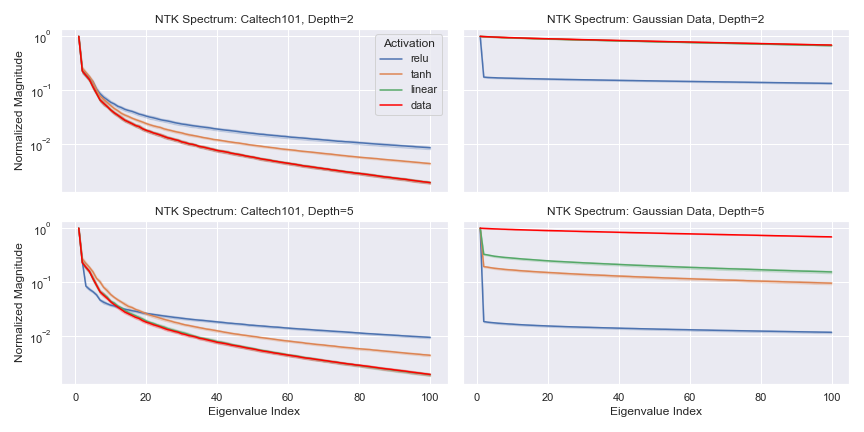
\includegraphics[width=\textwidth]{conference_files/images/fnn_spectrums2.png}
    \caption{\textbf{ (Feedforward NTK Spectrum) } We plot the normalized eigenvalues $\lambda_p / \lambda_1$ of the NTK Gram matrix $\mK$ and the data Gram matrix $\mX \mX^T$ for Caltech101 and isotropic Gaussian datasets. To compute the NTK we randomly initialize feedforward networks of depths $2$ and $5$ with width $500$. We use the standard parameterization and Pytorch's default Kaiming uniform initialization in order to better connect our results with what is used in practice. We consider a batch size of $n = 200$ and plot the first $100$ eigenvalues. The thick part of each curve corresponds to the mean across 10 trials, while the transparent part corresponds to the 95\% confidence interval}
    \label{fig:spectrum_cifar}
\end{figure}


\subsection{Analysis of the lower spectrum}\label{subsec:lower}
In this section, we analyze the lower part of the spectrum using the power series. 
We first analyze the kernel function $K$ which we recall is a dot-product kernel of the form $K(x_1,x_2) = \sum_{p = 0}^{\infty} c_p \langle x_1,x_2\rangle^p$. 
Assuming the training data is uniformly distributed on a hypersphere it was shown by \cite{uniform_sphere_data, bietti2019inductive} that the eigenfunctions of $K$ are the spherical harmonics. \cite{azevedo2015eigenvalues} gave the eigenvalues of the kernel $K$ in terms of the power series coefficients.
\begin{restatable}{theorem}{unifEigDecay}[\cite{azevedo2015eigenvalues}]\label{thm:eigen_hypersphere}  Let $\Gamma$ denote the gamma function.  Suppose that the training data are uniformly sampled from the unit hypersphere $\mathbb{S}^d$, $d\geq 2$.
If the dot-product kernel function has the expansion $K(x_1,x_2) = \sum_{p = 0}^{\infty} c_p \langle x_1,x_2\rangle^p$ where $c_p\geq 0$, then the eigenvalue of every spherical harmonic of frequency $k$ is given by 
\begin{equation*}
    \overline{\lambda_k}=\frac{\pi^{d/2}}{2^{k-1}}\sum_{\substack{p\geq k\\p-k\text{ is even}}}c_p\frac{ \Gamma(p+1)\Gamma(\frac{p-k+1}{2})}{\Gamma(p-k+1)\Gamma(\frac{p-k+1}{2}+k+d/2)}.
\end{equation*}
%where $\Gamma$ is the gamma function. 
\end{restatable} 

A proof of Theorem~\ref{thm:eigen_hypersphere} is provided in Appendix~\ref{appendix:lower_uniform} for the reader's convenience. This theorem connects the coefficients $c_p$ of the kernel power series with the eigenvalues $\overline{\lambda_k}$ of the kernel. In particular, given a specific decay rate for the coefficients $c_p$ one may derive the decay rate of $\overline{\lambda_k}$: for example, \cite{scetbon2021spectral} examined the decay rate of $\overline{\lambda_k}$ if $c_p$ admits a polynomial decay or exponential decay. The following Corollary summarizes the decay rates of $\overline{\lambda_k}$ corresponding to two layer networks with different activations.
\begin{restatable}{corollary}{ReLUbiaszero}\label{cor:ReLUbias0}
Under the same setting as in Theorem~\ref{thm:eigen_hypersphere}, 
\begin{enumerate}
    \item if $c_p = \Theta(p^{-a})$ where $a\geq 1$, then $\overline{\lambda_k} = \Theta(k^{-d-2a+2})$, 
    \item if $c_p = \delta_{(p \text{ even})} \Theta(p^{-a})$, then $\overline{\lambda_k} = \delta_{(k \text{ even})}\Theta(k^{-d-2a+2})$, 
    \item if $c_p = \cO\left(\exp\left( - a\sqrt{p}\right) \right)$, then $\overline{\lambda_k} = \cO\left(k^{-d+1/2}\exp\left( - a\sqrt{k}\right) \right)$, 
    \item if $c_p = \Theta(p^{1/2} a^{-p})$, then $\overline{\lambda_k} = \cO\left(k^{-d+1}a^{-k} \right)$ and $\overline{\lambda_k} =\Omega\left(k^{-d/2+1}2^{-k}a^{-k} \right)$. 
\end{enumerate}
\end{restatable} 
In addition to recovering existing results for ReLU networks \cite{uniform_sphere_data, NEURIPS2021_14faf969, geifman2020similarity, bietti2021deep}, Corollary~\ref{cor:ReLUbias0} also provides the decay rates for two-layer networks with Tanh and Gaussian activations. As faster eigenvalue decay implies a smaller RKHS Corollary \ref{cor:ReLUbias0} shows using ReLU results in a larger RKHS relative to Tanh or Gaussian activations. Numerics for Corollary \ref{cor:ReLUbias0} are provided in Figure~\ref{fig:asym_spectrum} in Appendix~\ref{appendix:subsection:emp_validation_ef}. Finally, in Theorem \ref{theorem:informal_ub_eigs_nonuniform} we relate a kernel's power series to its spectral decay for arbitrary data distributions. 

\begin{theorem}[Informal] \label{theorem:informal_ub_eigs_nonuniform}
    Let the rows of $\mX\in \reals^{n \times d}$ be arbitrary points on the unit sphere. Consider the kernel matrix $n\mK = \sum_{p=0}^{\infty} c_p \left(\mX \mX^T \right)^{\odot p}$ and let $r(n)\leq d$ denote the rank of $\mX\mX^T$. Then
    \begin{enumerate}
        \item 
        if $c_p = \cO(p^{-\alpha})$ with $\alpha > r(n)+1$ for all $n \in \ints_{\geq 0}$ then $\lambda_{n}(\mK) = \cO\left(n^{-\frac{\alpha-1}{r(n)}}\right)$,
        \item 
        if $c_p = \cO(e^{-\alpha \sqrt{p}})$ then $\lambda_{n}(\mK) = \cO \left(n^{\frac{1}{2r(n)}} \exp \left(-\alpha' n^{\frac{1}{2r(n)}} \right) \right)$ for any $\alpha' < \alpha 2^{-1/2r(n)}$,
        \item 
        if $c_p = \cO(e^{-\alpha p})$ then $\lambda_{n}(\mK) = \cO\left(\exp\left(-\alpha' n^{\frac{1}{r(n)}}\right)\right)$ for any $\alpha' < \alpha 2^{-1/2r(n)}$. 
    \end{enumerate}
\end{theorem}

Although the presence of the factor $1/r(n)$ in the exponents of $n$ in these bounds is a weakness, Theorem \ref{theorem:informal_ub_eigs_nonuniform} still illustrates how, in a highly general setting, the asymptotic decay of the coefficients of the power series ensures a certain asymptotic decay in the eigenvalues of the kernel matrix. A formal version of this result is provided in Appendix \ref{appendix:lower_non_uniform} along with further discussion.
